\documentclass[tikz,border=10pt]{standalone}
\begin{document}
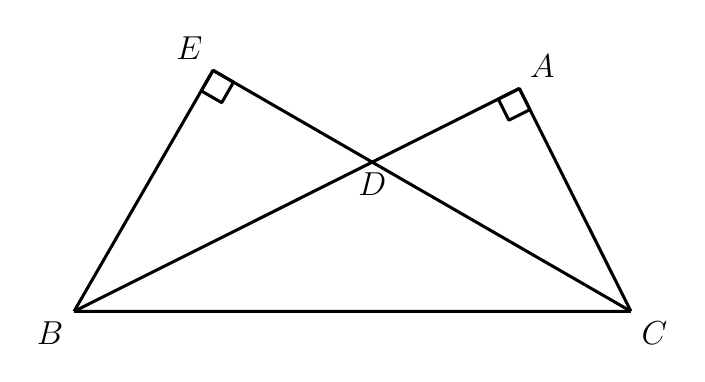
\begin{tikzpicture}[line join=round, line width=1.1pt]
  % Named points (scale s = 0.009988 cm/px, y flipped)
  \coordinate (B) at (-3.536334647434931,-1.531085904232202);
  \coordinate (C) at (3.5356116294113016,-1.5294538191337772);
  \coordinate (A) at (2.11922050570037,1.300009061759699);
  \coordinate (E) at (-1.7705379655775968,1.5307074355532182);
  \coordinate (D) at (0.25104047790085604,0.3648232260530621);

  % Segments (D lies on BA and EC, so they pass through D)
  \draw (B) -- (C);
  \draw (B) -- (E);
  \draw (E) -- (D) -- (C);
  \draw (B) -- (D) -- (A);
  \draw (A) -- (C);

  % Right-angle mark at A (between AB and AC), side 0.3 cm
  \draw (2.11922050570037,1.300009061759699) -- (1.8513976684109887,1.1656527984627088) -- (1.9855754305069322,0.8972393714764992) -- (2.2533982677963134,1.0315956347734894) -- cycle;

  % Right-angle mark at E (between EB and EC), side 0.3 cm
  \draw (-1.7705379655775968,1.5307074355532182) -- (-1.9201210193771623,1.2704657559928048) -- (-1.660349915031035,1.1200665314958944) -- (-1.5107668612314695,1.3803082110563076) -- cycle;

  % Labels
  \node[above right] at (A) {\fontsize{11.5}{13.8}\selectfont $A$};
  \node[below left]  at (B) {\fontsize{11.5}{13.8}\selectfont $B$};
  \node[below right] at (C) {\fontsize{11.5}{13.8}\selectfont $C$};
  \node[below]       at (D) {\fontsize{11.5}{13.8}\selectfont $D$};
  \node[above left]  at (E) {\fontsize{11.5}{13.8}\selectfont $E$};
\end{tikzpicture}
\end{document}